\documentclass{article}

\usepackage[UTF8]{ctex}
\usepackage{amsmath,amssymb}
\usepackage{geometry}
\usepackage{graphicx}

\geometry{a4paper, margin=2.5cm}

\begin{document}

% ============================================================
\section*{多臂老虎机问题（Multi-Armed Bandit, MAB）}

\subsection*{先讲一个故事}

你走进一家赌场，面前有 $K$ 台老虎机。每台老虎机有自己的中奖概率，但你完全不知道。你有 $T$ 次机会（每次一块钱），想最大化总奖金。

\textbf{核心困境}：把硬币投给哪台机器？
\begin{itemize}
  \item 投给「看上去不错的」—— 可能被前几次运气误导，永远错过真正的大奖机器；
  \item 每台都试一遍 —— 试差的机器纯属浪费。
\end{itemize}

这就是\textbf{探索（Exploration）vs.\ 利用（Exploitation）}的权衡，强化学习一切问题的源头。

\subsection*{数学形式化}

$K$-臂伯努利老虎机由以下要素定义：

\[
\boxed{\text{Bandit}_K = \{\mu_1, \mu_2, \ldots, \mu_K\}, \quad \mu_k \in [0,1]}
\]

\begin{itemize}
  \item $\mu_k$ —— 第 $k$ 个臂的真实中奖概率（\textbf{未知}）；
  \item 动作 $a_t \in \{1,\ldots,K\}$ —— 第 $t$ 步选择哪个臂；
  \item 奖励 $r_t \in \{0,1\}$ —— 拉完之后实际中的奖，$r_t \sim \text{Bernoulli}(\mu_{a_t})$；
  \item 最优臂 $\mu^* = \max_k \mu_k$，对应的臂编号 $k^* = \arg\max_k \mu_k$。
\end{itemize}

目标：在 $T$ 步内选动作序列 $(a_1,\ldots,a_T)$，最大化期望累积奖励 $\mathbb{E}\left[\sum_{t=1}^{T} r_t\right]$。

% ============================================================
\section*{懊悔 —— 衡量算法好坏的标尺}

\subsection*{定义}

最大化奖励等价于最小化\textbf{懊悔（Regret）}——你因为不知道哪个臂最好而损失了多少。

设第 $t$ 步选了臂 $a_t$，该步的\textbf{即时懊悔}为：
\[
\boxed{\rho_t = \mu^* - \mu_{a_t}}
\]

$T$ 步后的\textbf{累积懊悔}：
\[
\boxed{R(T) = \sum_{t=1}^{T} \rho_t = T\mu^* - \sum_{t=1}^{T} \mu_{a_t}}
\]

\subsection*{懊悔告诉我们什么}

\[
\begin{array}{c|c}
\text{懊悔增长速率} & \text{含义} \\
\hline
R(T) = O(T) \;\; \text{（线性）} & \text{算法没在学——每步都在犯错} \\
R(T) = O(\log T) \;\; \text{（对数）} & \text{算法在学习——犯错越来越少} \\
R(T) = O(\sqrt{T}) \;\; \text{（平方根）} & \text{介于两者之间} \\
\end{array}
\]

\textbf{Lai \& Robbins 下界（1985）}：任何一致算法（uniformly good，即对所有实例遗憾都亚线性）至少 $\Omega(\log T)$。注意 $O(\log T)$ 只是速率最优；匹配下界常数（$\sum_k \Delta_k / \mathrm{KL}(\mu_k,\mu^*)$）才是渐近最优。

% ============================================================
\section*{贪心策略与 $\varepsilon$-贪心}

\subsection*{纯贪心策略（Greedy）}

最朴素的想法：选当前估计最好的臂。
\[
a_t = \arg\max_k \hat{\mu}_k(t), \qquad
\hat{\mu}_k(t) = \frac{\text{臂 } k \text{ 历史上获得的总奖励}}{\text{臂 } k \text{ 被选中的总次数}}
\]

\textbf{致命缺陷}：第一次某个次优臂碰巧给了一个 $r=1$，被高估为 $\hat{\mu}_k = 1.0$。纯贪心永远不会再碰其他臂，永远卡在次优解。懊悔线性增长。

\subsection*{$\varepsilon$-贪心}

\textbf{核心思想}：大部分时间贪心（利用），小部分时间随机探索。

\[
a_t = \begin{cases}
  \text{随机选 } k \in \{1,\ldots,K\}, & \text{以概率 } \varepsilon \text{（探索）},\\[4pt]
  \arg\max_k \hat{\mu}_k(t), & \text{以概率 } 1-\varepsilon \text{（利用）}.
\end{cases}
\]

\subsection*{增量式均值更新（重要！）}

不需要存所有历史奖励。设已有 $N$ 次观测，均值为 $\hat{\mu}_N$，新观测 $r_{N+1}$ 到来时：

\[
\begin{aligned}
\hat{\mu}_{N+1} &= \frac{1}{N+1}\sum_{i=1}^{N+1} r_i
                 = \frac{1}{N+1}\left(r_{N+1} + \sum_{i=1}^{N} r_i\right) \\[4pt]
                &= \frac{1}{N+1}\left(r_{N+1} + N\hat{\mu}_N\right) \\[4pt]
                &= \frac{1}{N+1}\left(r_{N+1} + (N+1)\hat{\mu}_N - \hat{\mu}_N\right) \\[4pt]
                &= \hat{\mu}_N + \frac{1}{N+1}\left(r_{N+1} - \hat{\mu}_N\right).
\end{aligned}
\]

\[
\boxed{\hat{\mu}^{\text{new}} = \hat{\mu}^{\text{old}} + \frac{1}{N+1}\left(r - \hat{\mu}^{\text{old}}\right)}
\]

\textbf{为什么这个格式重要？} 它是\underline{整个 RL 更新规则的雏形}：
\[
\theta \leftarrow \theta + \alpha\,(\text{Target} - \theta)
\]
后面 Q-Learning 的 $Q(s,a) \leftarrow Q(s,a) + \alpha\,(r + \gamma\max Q - Q(s,a))$ 就是同一个结构。

\subsection*{常值 $\varepsilon$ 的遗憾分析}

固定 $\varepsilon > 0$，每一步以概率 $\varepsilon/K$ 选中任一特定臂。次优臂 $k$ 在 $T$ 步中期望被探索 $\frac{\varepsilon}{K}T$ 次，每次产生懊悔 $\Delta_k = \mu^* - \mu_k$。

\[
\mathbb{E}[R(T)] \ge \sum_{k: \Delta_k > 0} \frac{\varepsilon}{K}\,T \cdot \Delta_k = \frac{\varepsilon}{K}\,T\sum_k \Delta_k = \Omega(T)
\]

\textbf{结论}：常值 $\varepsilon$ 导致线性遗憾 —— 即使 $T \to \infty$，仍有 $\varepsilon$ 概率探索，一直浪费。

\subsection*{衰减 $\varepsilon$-贪心}

\textbf{改进}：让探索概率随时间衰减。$\varepsilon_t = 1/t$：
\[
\mathbb{P}(\text{第 } t \text{ 步探索}) = \frac{1}{t} \;\longrightarrow\; 0 \quad (t \to \infty)
\]

早期大量探索（$t$ 小时 $\varepsilon_t$ 大），后期专注利用。严格的对数遗憾保证需要足够大的衰减常数：取 $\varepsilon_t = cK/(d^2t)$（$d$ 为最小次优间隙，Auer et al.\ 2002）时遗憾为 $O(\log T)$；纯 $\varepsilon_t = 1/t$ 只保证亚线性遗憾，且匹配的是速率而非下界常数。

\textbf{注意}：$\varepsilon_t = c/t$ 的总探索次数约为 $c\ln T$，常数 $c$ 太小（如 $c=1$）时在有限步数内几乎不探索；实践中常给一个下界 $\varepsilon_{\min}$（如 $0.02$）保证足够的探索（见实验图~\ref{fig:optimal-arm}）。

\subsection*{乐观初始化}

另一个诱导探索的技巧：初始估值全部设为 $1.0$（最高可能值）。所有臂都被高估——拉一次后某臂估计下降，别的臂依然「虚高」，迫使算法轮流尝试所有臂。天然完成一轮探索后自动收敛到贪心。

% ============================================================
\section*{上置信界算法（UCB）}

\subsection*{$\varepsilon$-贪心的问题}

它的探索是\textbf{无方向}的——对所有臂一视同仁随机选，浪费大量机会在明显差的臂上。好的探索应该有方向：「我不确定这个臂好不好，所以试试它」。

\subsection*{核心思想：面对不确定性的乐观主义}

UCB 不只看点估计 $\hat{\mu}_k$，而是计算一个\textbf{置信上界}。不确定性越大的臂，上界被推得越高——即使它的点估计一般，也可能因为「万一是好的」而被选中。

\[
\boxed{a_t = \arg\max_k \left[\; \hat{\mu}_k(t) \;+\; \text{不确定性奖励} \;\right]}
\]

\subsection*{Hoeffding 不等式 —— 如何量化「不确定」}

设 $X_1,\ldots,X_n$ 为 $[0,1]$ 内独立同分布随机变量，$\bar{X}_n = \frac{1}{n}\sum_i X_i$，$\mu = \mathbb{E}[X_i]$。

\[
\boxed{\mathbb{P}\left(|\bar{X}_n - \mu| \ge \delta\right) \le 2\exp\left(-2n\delta^2\right)}
\]

\textbf{翻译成人话}：$n$ 次观测后，样本均值偏离真实期望 $\ge \delta$ 的概率以指数级缩小。

将这个不等式反过来用：给定置信度 $p$，解 $\exp(-2n\delta^2)=p$ 得到：
\[
\delta = \sqrt{\frac{\log(1/p)}{2n}}
\]

取 $p = 1/t$（随时间推移逐步收紧置信度），以概率 $\ge 1-2/t$：
\[
\mu_k \in \left[\hat{\mu}_k - \sqrt{\frac{\log t}{2 N_k}},\; \hat{\mu}_k + \sqrt{\frac{\log t}{2 N_k}}\right]
\]

选\textbf{上界}（乐观估计）：
\[
\boxed{a_t = \arg\max_k \left[\; \underbrace{\hat{\mu}_k(t)}_{\text{利用}} \;+\; \underbrace{c \cdot \sqrt{\frac{\log t}{2\,N_k(t)}}}_{\text{探索奖励}} \;\right]}
\]

\textbf{直觉}：
\begin{itemize}
  \item 臂被拉得多（$N_k$ 大）$\to$ 探索项小 $\to$ 上界收紧；
  \item 臂被遗忘（$N_k$ 小）$\to$ 探索项大 $\to$ 上界膨胀 $\to$ 被重新选中；
  \item $\log t$ 随步数 $t$ 极慢增长，保证长期来看探索代价很小。
\end{itemize}

$c$ 是控制探索/利用权衡的超参数。实际实现中常对 $N_k$ 加一平滑（$N_k+1$），防止除零并使未拉过的臂具有最大不确定性，保证所有臂至少被尝试一次。

\subsection*{遗憾上界（Auer et al.\ 2002）}

UCB1（$c=1$）的理论保证：
\[
\mathbb{E}[R(T)] \le 8\sum_{k: \mu_k < \mu^*} \frac{\log T}{\Delta_k} + C, \quad \text{即 } O(\log T)
\]
达到渐近最优。每个次优臂期望被拉 $\approx \frac{\log T}{\Delta_k^2}$ 次后，其置信区间窄到不可能再竞争，之后几乎遗忘。

% ============================================================
\section*{汤普森采样（Thompson Sampling）}

\subsection*{频率学派 vs.\ 贝叶斯学派}

前三个算法（Greedy、$\varepsilon$-Greedy、UCB）都是\textbf{频率学派}思路：根据历史数据算出一个点估计 $\hat{\mu}_k$，再围绕点估计加一些东西（噪音 / 置信界）。

汤普森采样是\textbf{贝叶斯学派}方法：不维护「一个数」，而是维护$\mu_k$的\textbf{完整概率分布}，表达「我对 $\mu_k$ 的信念是什么」。

\subsection*{Beta 分布与共轭先验}

伯努利试验的似然函数（观测到 $s$ 次成功、$f$ 次失败）：
\[
P(\text{data} \mid \mu) = \mu^{s}\,(1-\mu)^{f}
\]

Beta 分布的密度函数：
\[
\text{Beta}(\theta \mid \alpha, \beta) \propto \theta^{\alpha-1}(1-\theta)^{\beta-1}, \quad \theta \in [0,1]
\]

两者有相同的函数形式（$\mu$ 的幂乘 $(1-\mu)$ 的幂）。这意味着：

\textbf{如果先验是 Beta 分布，看到 Bernoulli 数据后，后验还是 Beta 分布}（共轭性）：

\[
\boxed{P(\mu \mid s \text{ 次成功, } f \text{ 次失败}) = \text{Beta}(\alpha_0 + s,\; \beta_0 + f)}
\]

取 $\alpha_0 = \beta_0 = 1$，$\text{Beta}(1,1) = \text{Uniform}(0,1)$，即「我一无所知」。

\subsection*{从先验到后验的推导}

\[
\begin{aligned}
P(\mu \mid r_{1:n}) &\propto P(r_{1:n} \mid \mu) \cdot P(\mu)  \\
&\propto \mu^{\sum r_i} (1-\mu)^{n-\sum r_i} \cdot \mu^{\alpha_0-1} (1-\mu)^{\beta_0-1} \\
&= \mu^{\alpha_0 + \sum r_i - 1}\,(1-\mu)^{\beta_0 + n - \sum r_i - 1} \\
&\propto \text{Beta}\left(\alpha_0 + \sum r_i,\; \beta_0 + n - \sum r_i\right).
\end{aligned}
\]

\textbf{Beta 分布随观测增多而变化}：

\[
\begin{array}{c|c|c}
\text{参数} & \text{含义} & \text{分布形状} \\
\hline
\alpha=1,\;\beta=1     & \text{无信息先验} & \text{均匀分布 } U[0,1] \\
\alpha=10,\;\beta=10   & 9\text{胜}9\text{负} & \text{集中在 } 0.5 \text{ 附近，较宽} \\
\alpha=80,\;\beta=20   & 79\text{胜}19\text{负} & \text{集中在 } 0.8 \text{ 附近，较窄} \\
\alpha=200,\;\beta=50  & 199\text{胜}49\text{负} & \text{集中在 } 0.8 \text{ 附近，更窄（很确定）} \\
\end{array}
\]

数据越多，分布越窄——你对 $\mu_k$ 的信念越确定。

实验观察：Thompson 采样各臂后验随数据收敛的过程如图~\ref{fig:thompson-posterior} 所示。

\begin{figure}[!htbp]
  \centering
  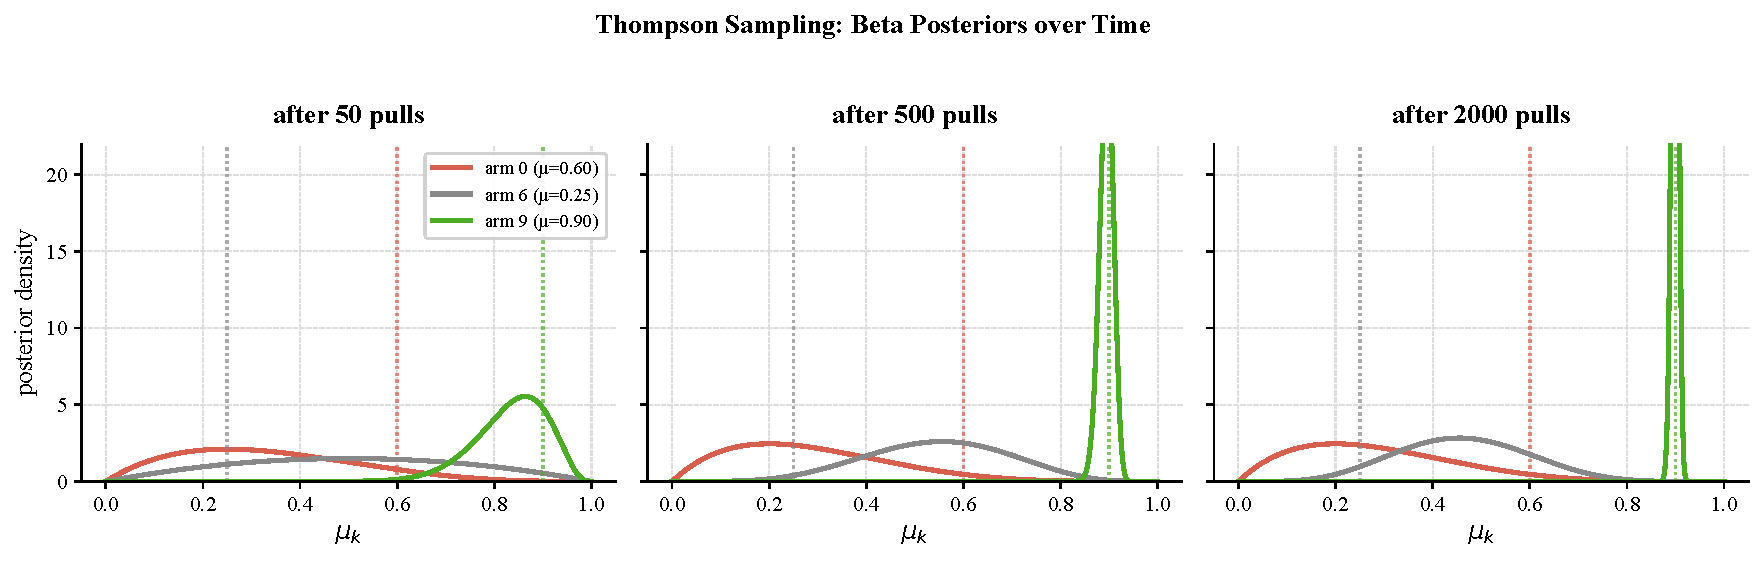
\includegraphics[width=0.92\textwidth]{fig3_thompson_posterior.pdf}
  \caption{Thompson 采样的后验演化（10 臂伯努利老虎机，最优臂 $\mu^*=0.90$，固定种子）。三个时刻（第 50 / 500 / 2000 步）三个臂的后验 $\mathrm{Beta}(\alpha_k,\beta_k)$：最优臂（绿）因被大量拉取而迅速收窄到 $0.90$ 附近；被冷落的次优臂（灰）长期保持“宽”的形态——后验宽度正是 Thompson 采样探索的驱动力。虚线标出各臂真实 $\mu_k$。}
  \label{fig:thompson-posterior}
\end{figure}

\subsection*{算法流程：三行搞定}

\begin{enumerate}
  \item \textbf{采样}：从每个臂的后验各采一个 $\tilde{\mu}_k \sim \text{Beta}(\alpha_k, \beta_k)$；
  \item \textbf{选}：$a_t = \arg\max_k \tilde{\mu}_k$（贪心选采样值最大的）；
  \item \textbf{更新}：$\alpha_{a_t} \leftarrow \alpha_{a_t} + r_t$，$\beta_{a_t} \leftarrow \beta_{a_t} + (1 - r_t)$。
\end{enumerate}

\subsection*{为什么「从后验采样再贪心」是对的？}

\textbf{概率匹配（Probability Matching）}：选择臂 $k$ 的概率，恰好等于「臂 $k$ 是最优臂」的后验概率。

\[
\mathbb{P}(a_t = k) = \mathbb{P}\big(\mu_k = \max_j \mu_j \mid \text{data}\big)
\]

\textbf{自动平衡探索与利用}：
\begin{itemize}
  \item 不确定性大的臂（Beta 分布宽）$\to$ 采样值波动大，有时很高 $\to$ 自然获得探索机会；
  \item 确定的差臂（Beta 分布窄集中在低值）$\to$ 几乎永远不会被采样超过好臂 $\to$ 浪费很少。
\end{itemize}

\subsection*{遗憾分析（Agrawal \& Goyal 2012）}

汤普森采样的期望累积遗憾也达到 $O(\log T)$；对 Bernoulli 情形，Kaufmann, Korda \& Munos（2012）进一步证明其渐近常数匹配 Lai \& Robbins 下界。在实践中它通常表现最好。

% ============================================================
\section*{四种算法对比总结}

实验验证（图~\ref{fig:regret} 与图~\ref{fig:optimal-arm}）：10 臂伯努利老虎机、20 个随机种子下，各算法的行为与本章理论吻合。

\begin{figure}[!htbp]
  \centering
  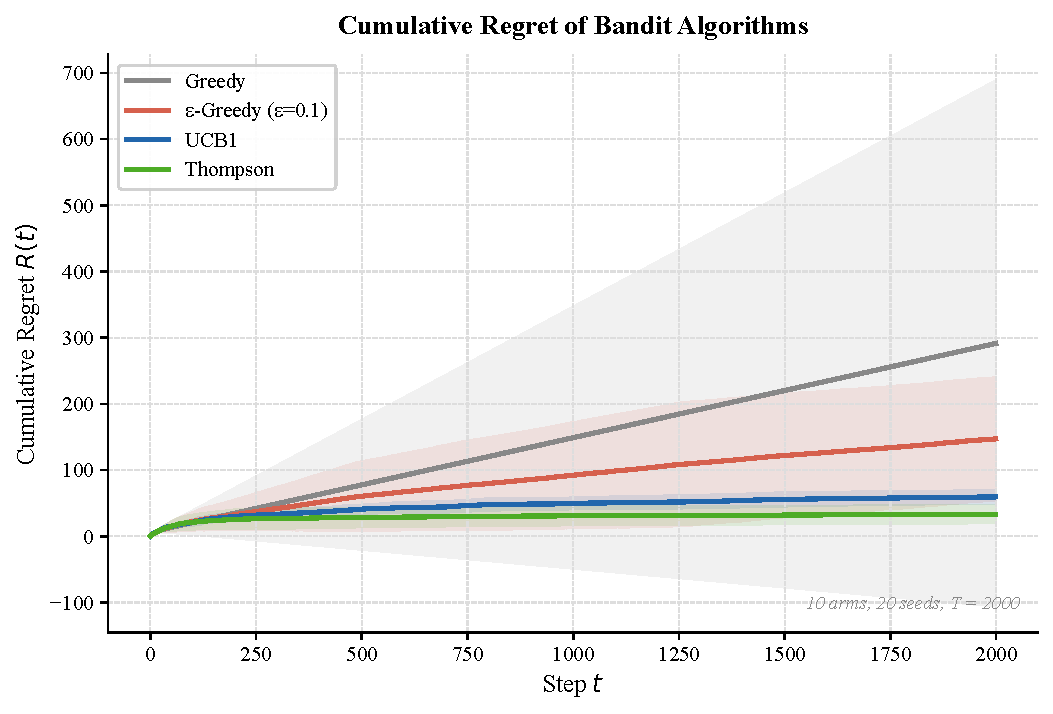
\includegraphics[width=0.88\textwidth]{fig1_regret_comparison.pdf}
  \caption{四种算法的累积懊悔 $R(T)$ 对比（20 个随机种子，阴影为 $\pm 1\sigma$）。Greedy 近似线性增长；$\varepsilon$-Greedy（$\varepsilon=0.1$）次之但仍是线性；UCB 与 Thompson Sampling 呈亚线性（$O(\log T)$）。}
  \label{fig:regret}
\end{figure}

\subsection*{探索方式的核心差异}

\begin{itemize}
  \item \textbf{$\varepsilon$-Greedy}：无差别随机探索。「规则让我随机试，我就随机试。」
  \item \textbf{UCB}：有方向探索。「我不确定 B 臂，万一它很好呢？给它一个机会。」
  \item \textbf{Thompson Sampling}：概率化探索。「我的信念是 B 臂有 30\% 概率最好，那么我有 30\% 的概率选它。」
  \item \textbf{Decaying $\varepsilon$-Greedy}：和 $\varepsilon$-Greedy 同类，但探索概率衰减。
\end{itemize}

从“把拉杆次数分配给最优臂的比例”也能看出各算法探索方式的不同，如图~\ref{fig:optimal-arm} 所示。

\begin{figure}[!htbp]
  \centering
  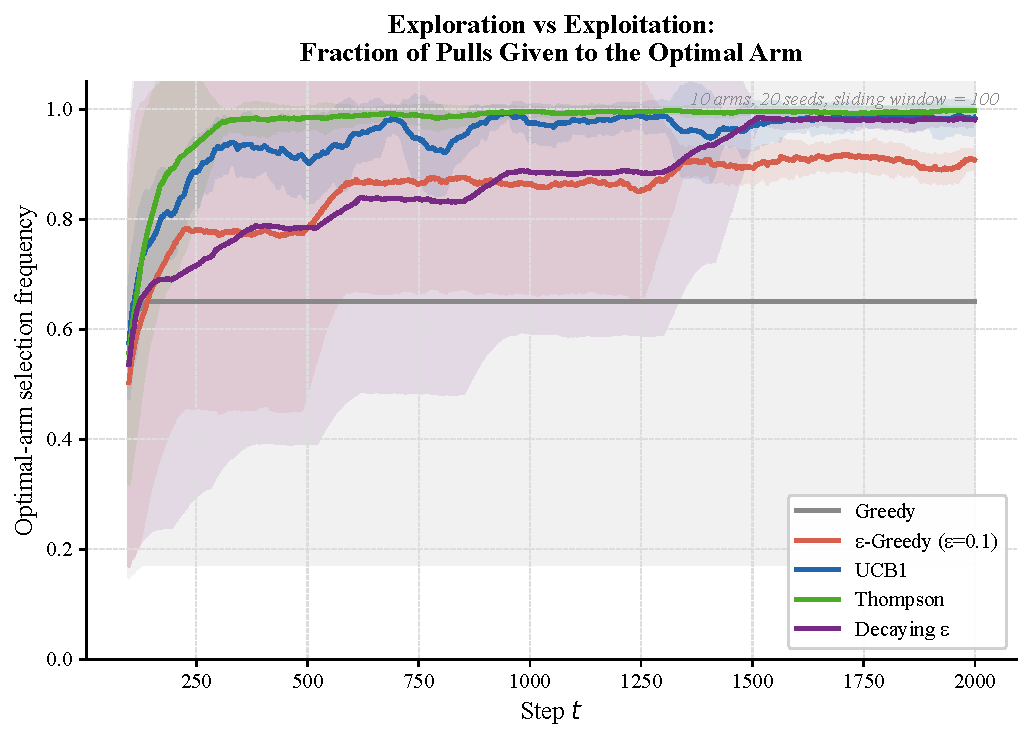
\includegraphics[width=0.88\textwidth]{fig2_optimal_arm_selection.pdf}
  \caption{各算法拉中最优臂的比例（20 个随机种子，100 步滑动平均，阴影为 $\pm 1\sigma$）。Greedy 每个种子只锁死一个臂，本例约三成种子被次优臂“困死”；$\varepsilon$-Greedy 停在 $1-\varepsilon=0.9$ 附近；衰减 $\varepsilon$ 缓慢爬向 1；UCB 与 Thompson Sampling 收敛最快。}
  \label{fig:optimal-arm}
\end{figure}

\subsection*{一表打尽}

\[
\begin{array}{c|c|c|c}
\text{算法} & \text{探索方式} & \text{理论遗憾} & \text{特点} \\
\hline
\varepsilon\text{-Greedy}      & \text{随机均匀} & O(T)\text{（线性）}          & \text{最简单，但遗憾不收敛} \\
\text{Decaying-}\varepsilon     & \text{随机均匀，概率衰减} & O(\log T)\text{（需调 } c\text{）} & \text{简单改进} \\
\text{UCB}                      & \text{有方向（置信界）}  & O(\log T)           & \text{确定性，调参简单} \\
\text{Thompson Sampling}        & \text{有方向（后验采样）} & O(\log T)\text{ 最优常数} & \text{实践中最强} \\
\end{array}
\]

\subsection*{实际选择建议}

\begin{enumerate}
  \item 快速原型 / 教学：$\varepsilon$-Greedy 或 Decaying $\varepsilon$-Greedy。
  \item 需要理论保证 + 调参少：UCB（仅 $c$ 一个参数）。
  \item 实际应用（推荐系统、广告投放、A/B 测试）：\textbf{Thompson Sampling}，通常表现最好，且能自然融入领域知识作先验。
\end{enumerate}

% ============================================================
\section*{本章在 RL 体系中的位置}

MAB 是单状态的强化学习。理解了本章，你就握住了 RL 三个核心概念的种子：

\begin{enumerate}
  \item \textbf{探索 vs.\ 利用} —— MAB 是最纯粹的形式；MDP 中变成「探索哪个状态-动作对」，同构问题。
  \item \textbf{增量更新} $\theta \leftarrow \theta + \alpha(\text{Target} - \theta)$ —— 这是 TD 学习、Q-Learning、Policy Gradient 的统一更新骨架。
  \item \textbf{不确定性驱动的探索} —— UCB $\to$ count-based exploration $\to$ RND（Random Network Distillation），一路演化；Thompson Sampling $\to$ PSRL（Posterior Sampling RL），是 Bayesian RL 的起点。
\end{enumerate}

下一章 MDP 把「单状态」扩展为「状态转移」，加上 Markov 性质和 Bellman 方程，整个 RL 的理论大厦就立起来了。

\subsection*{参考资料}

\begin{enumerate}
  \item Sutton \& Barto (2018). \textit{Reinforcement Learning: An Introduction} (2nd ed.). Chapter 2.
  \item Lai \& Robbins (1985). Asymptotically efficient adaptive allocation rules. \textit{Advances in Applied Mathematics}.
  \item Auer, Cesa-Bianchi \& Fischer (2002). Finite-time analysis of the multiarmed bandit problem. \textit{Machine Learning}.
  \item Agrawal \& Goyal (2012). Analysis of Thompson sampling for the multi-armed bandit problem. \textit{COLT}.
  \item Kaufmann, Korda \& Munos (2012). Thompson Sampling: An Asymptotically Optimal Finite-Time Analysis. \textit{ALT}.
  \item 动手学强化学习（Hands-on-RL）. 第2章：多臂老虎机.
\end{enumerate}

\end{document}
